\documentclass[titlepage]{article}
\usepackage[utf8]{inputenc}
\usepackage{fancyhdr}
\usepackage{titling}
\usepackage{tabto}
\usepackage[ddmmyyyy]{datetime}
\usepackage{graphicx}
\renewcommand{\dateseparator}{.}
\renewcommand{\figurename}{Obr.}
\graphicspath{ {/home/andras/Documents/kop/img/} }
\title{\textbf{Jednozvodový elektrokardiograf} \\
\large Praktická časť odbornej zložky maturitnej skúšky}
\date{\empty}

\begin{document}

\bgroup
	\fancypagestyle{empty} {
		\fancyhead[C] {Stredná priemyselná škola elektrotechnická S. A. Jedlika v Nových Zámkoch}
		\fancyfoot[L] {
			\begin{flushleft}
				Nové Zámky, 2018
			\end{flushleft}		
		}
		\fancyfoot[R] {
			\begin{flushright}
				riešiteľ: \textbf{András Zemes} \\
				ročník štúdia: \textbf{štvrtý}
			\end{flushright}
		}
		\fancyfoot[C] {\empty}		
	}
	\maketitle
\egroup


\section*{Praktická časť odbornej zložky maturitnej skúšky}
\underline{Zadanie úlohy pre komplexnú maturitnú skúšku:} 
\newline

\begin{description}
	\item [Meno a priezvisko:]
		\tabto{4cm} András Zemes
		
    \item [Trieda:]	
    	\tabto{4cm} 4. IT
    	
	\item [Konzultant:]		 	  
		\tabto{4cm} Mgr. Peter Hudec
		
	\item [Skolský rok:] 
		\tabto{4cm} 2018/2019
		
	\item [Odbor:]		  
		\tabto{4cm} Informačné a sieťové technológie
		
	\item [Názov témy:]			  
		\tabto{4cm} Jednozvodový elektrokardiograf 
		
	\item [Úloha:]				  
		\tabto{4cm} Zhotoviť prístroj, \emph{elektrokardiograf}, na snímanie 
		\tabto{4cm} a zachytenie elektrických potenciálov srdca.
		
	\item [Špecifikácia úlohy:] \hfill
	
    \begin{enumerate}
		\item Naštudovanie a spracovanie potrebnej teórie
		\begin{itemize}
			\item Elektrický potenciál srdca
        	\item Prehľad prístrojov EKG
        	\item Signál a jeho spracovanie
		\end{itemize}
    	\item Vytvorenie a konštrukcia prístroja na meranie EKG
    	\item Vytvorenie elektronickej časti, práca s mikrokontrolérom
    	\item Vytvorenie PC aplikácie na grafické zobrazenie spracovaných údajov
    	\item Webové rozhranie ku spracovaným dátam
	\end{enumerate}
	
	\item [Praktický charakter úlohy:]
		Návrh plošného spoja, programovanie 
		\tabto{4cm} mikrokontroléra, vytvorenie grafickej aplikácie.
		
\end{description}
	
\vspace{10mm}
\hrulefill
\\\hspace*{0mm}\phantom{v.r.: }András Zemes, riešiteľ

\vspace{10mm}
\hrulefill
\\\hspace*{0mm}\phantom{v.r.: }Mgr. Peter Hudec, interný konzultant

\vspace{10mm}
\hrulefill
\\\hspace*{0mm}\phantom{v.r.: }Zástupkyňa riaditeľa školy

\vspace{15mm}
V Nových Zámkoch dňa \today


\section*{Čestné vyhlásenie}

Ja, dolupodpísaný András Zemes, študent 4. IT triedy Strednej priemyselnej školy S. A. Jedlika v Nových Zámkoch, týmto vyhlasujem, že som túto prácu   vyhotovil sám, s použitím uvedenej literatúry a podľa rád môjho konzultanta. 

\vspace{10mm}
\hrulefill
\\\hspace*{0mm}\phantom{v.r.: }András Zemes
\newpage

\section*{Poďakovanie}
Touto cestou by som sa chcel poďakovať všetkým, ktorí mi akýmkoľvek spôsobom pomohli a povzbudzovali ma pri vypracovaní mojej komplexnej maturitnej práce. Predovšetkým však patrí moja vďaka konzultantovi, Mgr. Petrovi Hudecovi, za jeho všestrannú pomoc, za vedenie a cenné pripomienky pri záverečnom spracovaní práce.


\newpage
\section{Princíp fungovania EKG}
\subsection{Elektrofyziológia srdca}

Základom vnútorného fungovania srdca je jeho elektrická aktivita. Srdce je jedinečný orgán z hľadiska, že jeho elektrická činnosť nie je nervovo založená. Je riadená špecializovanými vodivými svalovými bunkami. Zväzky takýchto buniek podmieňujú čerpaciu schopnosť srdca.

Zdrojom elektrických impulzov je sinoatriálny (SA) uzol, ktorý sa nachádza v stene hornej časti pravej predsiene. Udáva frekvenciu kontrakcií myokardu (srdcového svalstva), ktorá je nominálne 70 tepov za minútu.

Signály sa ďalej šíria vodivými dráhami predsiení a stimulujú svalové kontrakcie. Pokračujú po srdcovej priehradke, septe, ktorá oddeľuje dve polovice srdca. Blízko bodu spojenia štyroch dutín srdca sa nachádza zhluk špeciálnych buniek - atrioventrikulárny (AV) uzol. Uzol AV postup vzruchov mierne inhibuje a následne ich vysiela do Hisovho zväzku.

Hisov zväzok  sa delí na dve vetvy, tzv. Tawarove ramienka. Obidve vetvy vedú do siete Purkyňových vláken, ktoré aktivujú pracovný myokard.
\\
\\

\begin{figure}[!ht]
\begin{center}
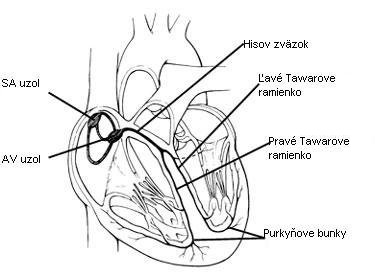
\includegraphics[scale=0.7]{48_img1_b}
\caption{Prevodový systém srdca}
\end{center}
\end{figure}

\newpage
\subsection{Akčný potenciál}
Ako vyrába a prenáša srdcové tkanivo elektrické impulzy? Aby sme si priebeh tohto deja mohli vysvetliť, musíme sa preniesť až na úroveň atómov.

\emph{Atóm je neutrálny,} ak má rovnaký počet protónov (kladne nabitých častíc) a elektrónov (záporne nabitých častíc). 

\emph{Ióny vznikajú} z elektricky neutrálnych atómov pridaním resp. ubraním elektrónov. 

V pokoji je srdcová bunka v \emph{polarizovanom stave}:
\begin{itemize}
	\item mimobunkový priestor je elektricky pozitívny pre vysokú koncentráciu kladných iónov sodíka a vápnika
	\item vnútrobunkový priestor je oproti vonkajšej strane negatívny
	\item rozdiel potenciálov je -90mV
\end{itemize}

Keď pokojový membránový potenciál dosiahne určitú prahovú hodnotu (cca. 15 mV), tzv. \emph{akčný potenciál}, tento pokojový stav sa náhle zmení. V membráne bunky sa otvoria prieduchy a kladne nabité ióny prúdia späť do bunky. Táto náhla strata polarizácie sa volá depolarizácia a vzniká pri nej elektrický prúd.

Po depolarizácii nastáva protikladný dej, repolarizácia, keď sa ióny znovu prečerpávajú von mimo membránu. Depolarizačná vlna vyvolávaná uzlom SA sa šíri po prevodovom systéme srdca a uvádza svaly do pohybu. Proces, ktorý začal pumpovaním iónov takto končí pumpovaním krvi. 

\begin{figure}[!ht]
\begin{center}
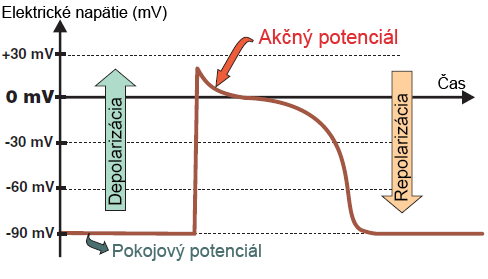
\includegraphics[scale=0.5]{action-potential-voltage}
\caption{Akčný potenciál v grafickom vyobrazení}
\end{center}
\end{figure}

%https://www.jfmed.uniba.sk/fileadmin/jlf/Pracoviska/ustav-patologickej-fyziologie/07Pregradualne_studium/01Vseobecne_lekarstvo/04Handouty_a_prednasky/01Handouty/01Elektrokardiografi1-jun10.pdf

\newpage
\subsection{Umiestnenie elektród}
Tri končatinové elektródy (pravá ruka, ľavá ruka, ľavá noha)  vytvárajú Einthovenov trojuholník. Vzniknú 3 \emph{bipolárne zvody} reprezentované stranami trojuholníka. Každý zvod pozostáva z dvoch elektród, z pozitívneho a z negatívneho. Pozitívny a negatívny pól spolu tvoria elektrický vektor, ktorý sa premieta na papier.

\begin{description}
	\item Zvod I: \tabto{1cm} $V_{I} = \phi_L - \phi_R$
	\item Zvod II: \tabto{1cm} $V_{II} = \phi_F - \phi_R$
	\item Zvod III:	\tabto{1cm} $V_{III} = \phi_F - \phi_L$
\end{description}
, kde: \\
\tabto{1cm} $V_{I}$ = napätie zvodu I\\
\tabto{1cm} $V_{II}$ = napätie zvodu II\\
\tabto{1cm} $V_{III}$ = napätie zvodu III\\
\tabto{1cm} $\phi_L$ = potenciál na ľavej ruke\\
\tabto{1cm} $\phi_R$ = potenciál na pravej ruke\\
\tabto{1cm} $\phi_F$ = potenciál na ľavej nohe\\
\\
Podľa Kirchhoffovho zákona platí, že veľkosť potenciálov (amplitúd na EKG zázname) v zvode $V_{II}$ je sumou potenciálov v zvodoch $V_{I}$ a  $V_{III}$:
\tabto{1cm} $V_{I} + V_{III} = V_{II}$
, z čoho vyplýva, že iba dva z troch zvodov sú nezávislé.
\\
\\
Einthoven definoval rozdiely potenciálov medzi troma pármi horeuvedených bodov ako základné končatinové zvody v elektrokardiografii.


\begin{figure}[!ht]
\begin{center}
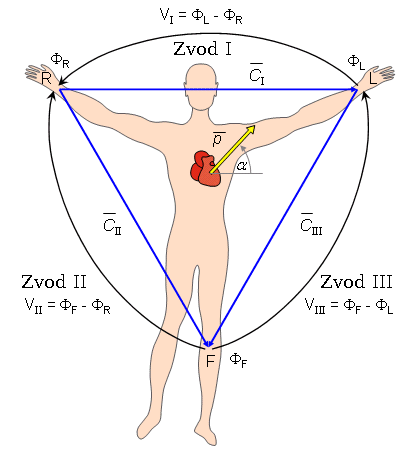
\includegraphics[scale=0.4]{ekg-zvody}
\caption{Einthovenove končatinové zvody a Einthovenov trojuholník}
\end{center}
\end{figure}
%http://www.bem.fi/book/15/15.htm


\newpage 
\subsection{Prehľad prístrojov EKG}


\newpage
\section*{Problematika a prehľad literatúry}
Srdcovú činnosť umožňujú malé elektrické impulzy, ktoré sa šíria po prevodovom systéme a pracovnom myokarde. Menia elektrické potenciály na rôznych bodoch pokožky približne o tisícinu voltu (1 mV). Táto elektrická aktivita v sebe skrýva neuveriteľné množstvo informácií, prostredníctvom ktorých môžeme získať náhľad do fungovania tohto zázračného orgánu.

K zachyteniu a odhaleniu signálu sa našťastie žiadne špeciálne vybavenie nevyžaduje. Odmerať ho dokážeme aj jednoduchým prístrojom vyrobeným doma.

Výzvou pokusu je spoľahlivo zosilniť pomerne slabý, milivoltový signál meniaci sa každú stotinu sekundy. 



\newpage
\section*{Ciele}
Kľúč úspešného elektrotechnického projektu spočíva v dokonalom zosúladení jeho elektronických a informačných zložiek. Zámerom tejto práce je poukázať na to, že aj pomerne jednoduchými komponentmi sa dajú vyriešiť komplexné problémy. 

Dôležité aspekty výslednej práce sú univerzálnosť, portabilita a intuitívny dizajn. Prístroj by mal vedieť použiť každý bez špeciálneho vybavenia a bez podrobnej znalosti jeho fungovania. Riešenie má byť taktiež prenosné, aby bolo neobmedzene využiteľné.

Pri návrhu plošného spoja sa muselo prihliadať i na bezpečnosť pri použití prístroja. Elektrokardiograf sleduje pulz snímaním elektrických potenciálov srdca z povrchu tela elektródami. Izoláciou elektród od zdroja sa zabránilo výskytu nečakaných a potenciálne rizikových situácií.

Pomocou jednozvodového EKG vieme určiť pulz, srdcový rytmus, ba aj odhaliť prítomnosť srdových arytmií a fibrilácie predsiení. Projekt môže taktiež slúžiť ako pomôcka pri výučbe elektroniky, programovania či informatiky. Znázorňuje fungovanie signálových filtrov, operačných zosilňovačov, mikrokontrolérov a grafických počítačových aplikácií.

\newpage
\section*{Prvý prototyp zosilňovacieho obvodu}
Ku dňu 15.10.2018 som na vývojovej doske zostavil funkčný prototyp zosilňovacieho obvodu elektrokardiografu. Z bezpečnostných dôvodov je zdrojom elektrického obvodu 9V batéria. Operačný zosilňovač LM741 slúži na zosilnenie nízkonapäťového vstupu z elektród priložených na povrch tela. 

Analógový výstup je spracovaný pomocou analógovo-digitálneho prevodníka zvukovej karty počítača. Signál softvérovo filtruje a graficky zobrazuje počítačová aplikácia.

Ďalším krokom je osamostatniť AD prevod signálu prostredníctvom mikrokontroléra. Aby sa to mohlo uskutočniť, zosilnený signál s negatívnou napäťovou zložkou sa musí premapovať  na rozsah kompatibilný s prevádzkovým rozsahom napätia mikrokontroléra.

Hlavnou problematikou tohto návrhu je výskyt elektromagnetickej interferencie v meraných hodnotách. Na minimalizáciu rušivých faktorov sa môže použiť pasívny RC dolnopriepustný filter.

\newpage
\section*{Zoznam použitej literatúry}
\begin{itemize}
\item 1991. Ľudské telo - Komplexný sprievodca po ľudskom tele a jeho funkciách. Bratislava. GEMINI, spol. s.r.o. ISBN 80-85265-12-5.
\item IAIZZO, Paul A. 2005. Handbook of Cardiac Anatomy, Physiology, and Devices. New Jersey. Human Press, Inc. ISBN 1-59259-835-8.
\item HANÁČEK, Ján, PLEVKOVÁ, Jana. 2009. Elektrokardiografia - Základné mechanizmy porúch elektrickej funkcie srdca a ich manifestácia na Ekg krivke. Martin. Ústav patologickej fyziológie JLF UK.
\item MALMIVUO, Jaakko, PLONSEY, Robert. 1995. Bioelectromagnetism - Principles and Applications of Bioelectric and Biomagnetic Fields. Oxford. Oxford University Press.
\item https://www.swharden.com/wp/2016-08-08-diy-ecg-with-1-op-amp/
\item https://www.kardiolog.sk/o-srdci/
\item https://www.techmed.sk/akcny-potencial/

\end{itemize}


\end{document}